\documentclass[a4paper]{article} 
\addtolength{\hoffset}{-2.25cm}
\addtolength{\textwidth}{4.5cm}
\addtolength{\voffset}{-3.25cm}
\addtolength{\textheight}{5cm}
\setlength{\parskip}{0pt}
\setlength{\parindent}{0in}

\usepackage[square,sort,comma,numbers]{natbib}
\usepackage{blindtext} % Package to generate dummy text
\usepackage{charter} % Use the Charter font
\usepackage[utf8]{inputenc} % Use UTF-8 encoding
\usepackage{microtype} % Slightly tweak font spacing for aesthetics
\usepackage{amsthm, amsmath, amssymb} % Mathematical typesetting
\usepackage{float} % Improved interface for floating objects
\usepackage{hyperref} % For hyperlinks in the PDF
\usepackage{graphicx, multicol} % Enhanced support for graphics
\usepackage{xcolor} % Driver-independent color extensions
\usepackage{pseudocode} % Environment for specifying algorithms in a natural way
\usepackage[mmddyy]{datetime} % Uses YEAR-MONTH-DAY format for dates

\usepackage{fancyhdr} % Headers and footers
\pagestyle{fancy} % All pages have headers and footers
\fancyhead{}\renewcommand{\headrulewidth}{0pt} % Blank out the default header
\fancyfoot[L]{} % Custom footer text
\fancyfoot[C]{} % Custom footer text
\fancyfoot[R]{\thepage} % Custom footer text
\newcommand{\note}[1]{\marginpar{\scriptsize \textcolor{red}{#1}}} % Enables comments in red on margin

\DeclareMathOperator*{\argmin}{arg\,min}

%----------------------------------------------------------------------------------------


%-------------------------------
%	TITLE VARIABLES (identify your work!)
%-------------------------------

\newcommand{\yourname}{Balthazar Neveu | Jamy Lafenetre}
\newcommand{\youremail}{balthazarneveu@gmail.com | jamy.lafenetre@ens-paris-saclay.fr}
\newcommand{\assignmentnumber}{5}

\begin{document}

%-------------------------------
%	TITLE SECTION (do not modify unless you really need to)
%-------------------------------
\fancyhead[C]{}
\hrule \medskip
\begin{minipage}{0.295\textwidth} 
\raggedright
\footnotesize
\yourname \hfill\\
\youremail
\end{minipage}
\begin{minipage}{0.4\textwidth} 
\centering 
\large 
Lab session \# \assignmentnumber\\ 
\normalsize 
NPM 2024\\ 
\end{minipage}
\begin{minipage}{0.295\textwidth} 
\raggedleft
\today\hfill\\
\end{minipage}
\medskip\hrule 
\bigskip




%-------------------------------
%	ASSIGNMENT CONTENT (add your responses)
%-------------------------------


\section*{Question 1}

The best segmentation we got was using a minimum number of points of 2000 per plane, a minimum distance of 0.1, a sampling resolution of 0.2, a max normal deviation of 10 degrees and an overlooking probability of 0.01.
The resulting segmentation was composed of 56 planes, as can be seen on figure \ref{fig:Q1}.

\begin{figure}[ht]
    \centering
    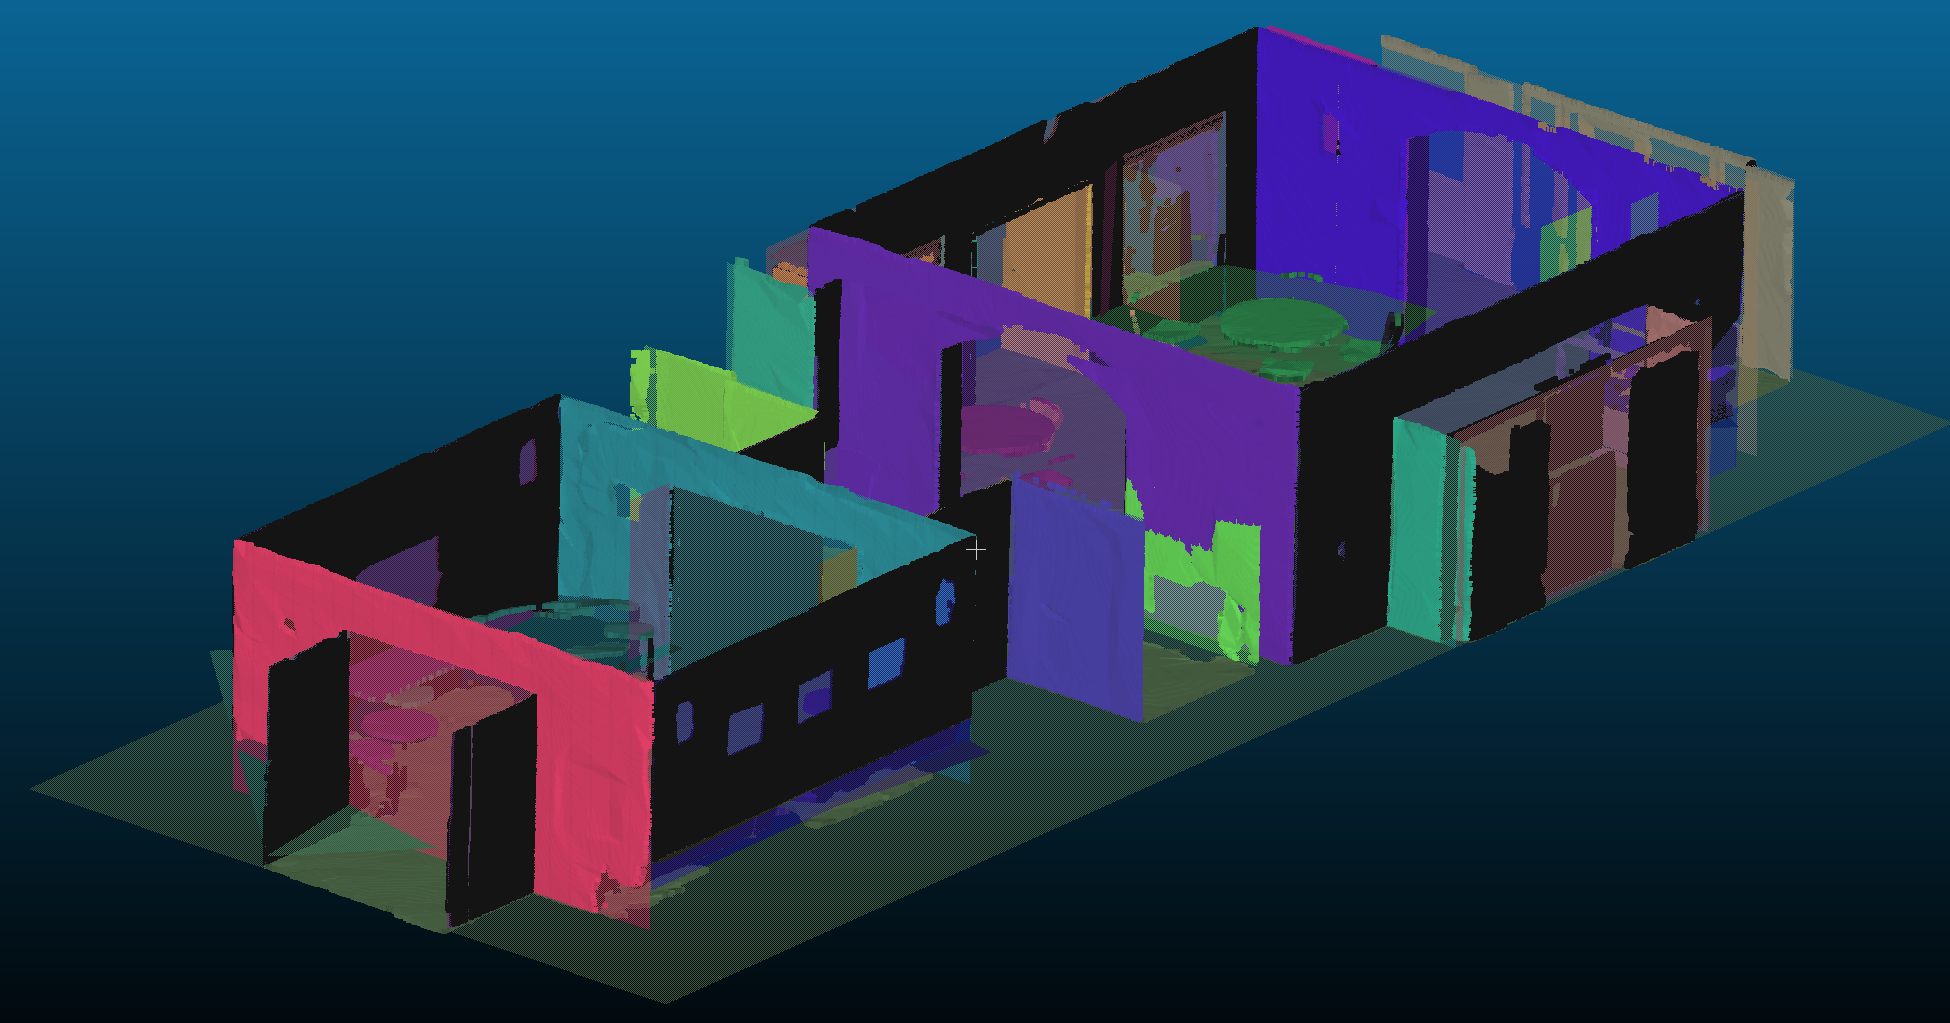
\includegraphics[width=0.3\linewidth]{figures/Q1.png}
    \caption{Result of the CloudCompare segmentation.}
    \label{fig:Q1}
\end{figure}


\section*{Question 2}

This result is undesirable because the second plan is not a good representaion of the point cloud. It does not represent any underlying plane structure,
but still managed to get the maximum ammount of votes by simply cutting the vertical axis. This highlights that a vote based on the distance criterion alone is not sufficient, especially 
when the samples are distributed radially. This can be seen on Figure \ref{fig:Q2}.

\begin{figure}[ht]
    \centering
    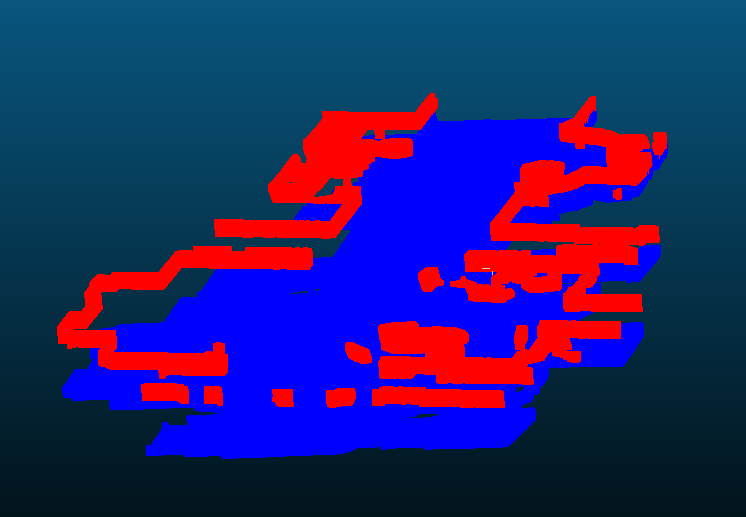
\includegraphics[width=0.3\linewidth]{figures/Q2.png}
    \caption{The distance criterion alone is not sufficiant for the indoor scene.}
    \label{fig:Q2}
\end{figure}

\section*{Question 3}

We evaluate the same algorithm on "Lille_street" from previous assignments. We use 2 planes, a distance threshold of 0.1 and 200 draws.
The segmentation gives better results on this scene, because the point distribution is not radially distributed as in the indoor cloud point. This can be seen on figure \ref{fig:Q3}.

\begin{figure}[ht]
    \centering
    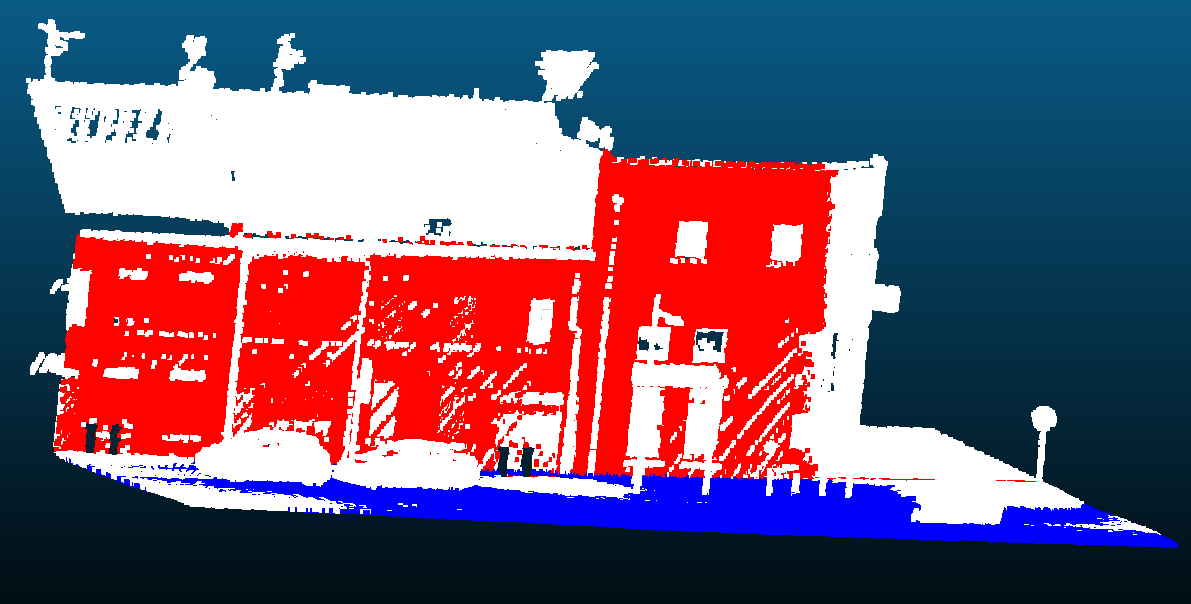
\includegraphics[width=0.3\linewidth]{figures/Q3.png}
    \caption{For Lille_street, the distance criterion is more satisfactory (for 2 planesat least).}
    \label{fig:Q3}
\end{figure}

\section*{Question 4}

To avoid the previous pitfalls, we can enrich the voting criterion by estimating the normals of the point cloud using a local PCA. Instead of proposing
a plane by picking 3 random samples, we can instead pick a single sample and its associated normal. Then, candidate points will only vote if they satisfy the distance criterion, as well
as a criterion measuring the angle difference between their normal and the proposed plane normal.
There are two major improvements to this strategy:
\item First, the candidate planes are far superior to what we had before, because they are locally optimal. Ransac should therefore converge in fewer iterations.
\item Second, points can only be considered as inliers of a plane if the local geometry resembles the plane. This will strongly reject planes that intersect every structure.

By doing so, the segmentation is considerably better, as can be seen on figure \ref{fig:Q4}.

\begin{figure}[ht]
    \centering
    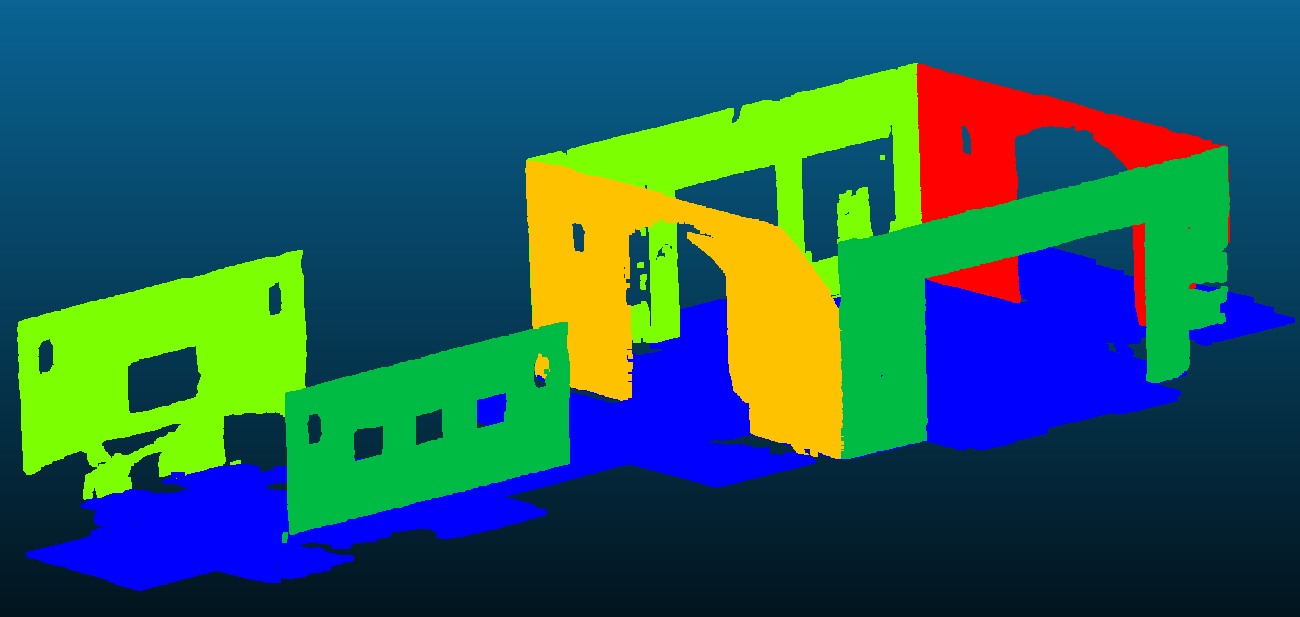
\includegraphics[width=0.3\linewidth]{figures/Q4.png}
    \caption{Segmentation with 5 planes, using a distance thrshold 0.2, an angle threshold of 10 degrees and 500 draws.
    Adding a criterion on the angle between the normals and the plane significantly improves the segmentation.}
    \label{fig:Q4}
\end{figure}

\section*{Bonus}
Our Ransac implementation is already quite fast and takes around than 10 seconds to run on GPU.
This is because we treat every candidate plane in parallel, instead of treating them one by one. Let's pretend in what follows that we do it in series (in a "for" loop).

A first source of optimisation is to drop the fixed number of iteration $N_{iter}$, and replace it with a fixed probability $1 - \beta$ of convergence.
We will instead dynamically update $N_iter$ based on the best vote found so far.
We call "inliers" points that vote positively for a candidate plane. By noting $m$ the (unknown) exact total amount of inliers,
the objective is to iterate until the total probability of picking the righ plane among the $N$ is more than $1 - \beta$. In other words :

$$
(1 - m/N)^N_{iter} \leq \beta
$$

Which can be written as 
$$
N_{iter} \geq \frac{log(\beta)} {log(1-m/N)}
$$


The trick is to notice that, although $m$ is unknown, the best estimated number of inliers so far is a lower bound of it. We can therefore dynamically reduce $N_{iter}$ as we iterate.
A second (smaller) source of optimisation is to only check the angle threshold condition if the distance threshold condition is satisfied.

These tricks are however mainly designed for CPU computing, as they cannot use the SIMD computation power brought by GPUs. To further use the available hardware, we compute $B$ regular ransac iterations at the same time, therefore simultaneously evaluating multiple planes.
We empirically found that, for this specific point cloud and for the specific case of segmentation by planes, $B=5$ was optimal to minimize the overhead.
With $\beta = 0.01$ and $B=5$, we managed to make a 5-planes segmentation in 0.92 seconds. The quality result with and without the optimisation trick are near identical, as can be seen on figure \ref{fig:bonus}, but the speedup is considerable as can be seen on
\ref{fig:bonus_1}

\begin{figure}[ht]
    \centering
    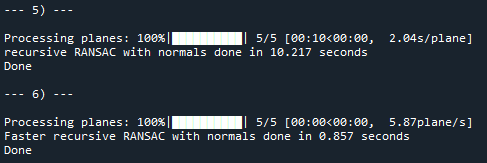
\includegraphics[width=0.3\linewidth]{figures/bonus.png}
    \caption{Esxecution time of the original and improved Ransac.}
    \label{fig:bonus_1}
\end{figure}

\begin{figure}[ht]
    \centering
    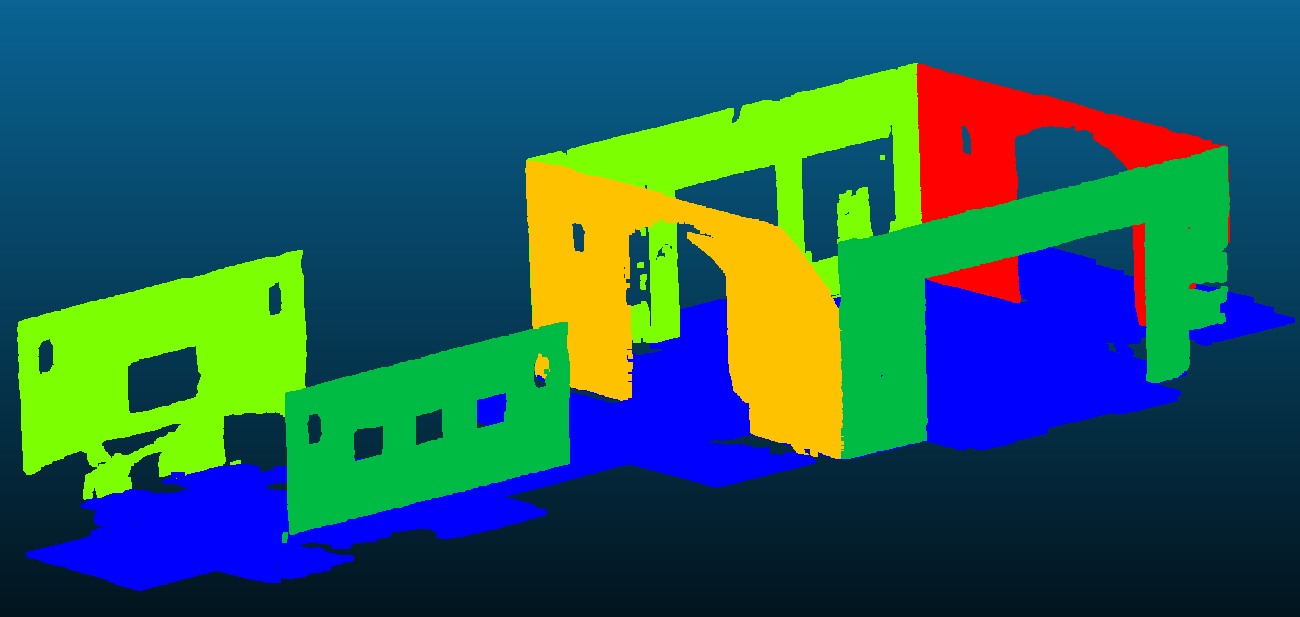
\includegraphics[width=0.3\linewidth]{figures/Q4.png}
    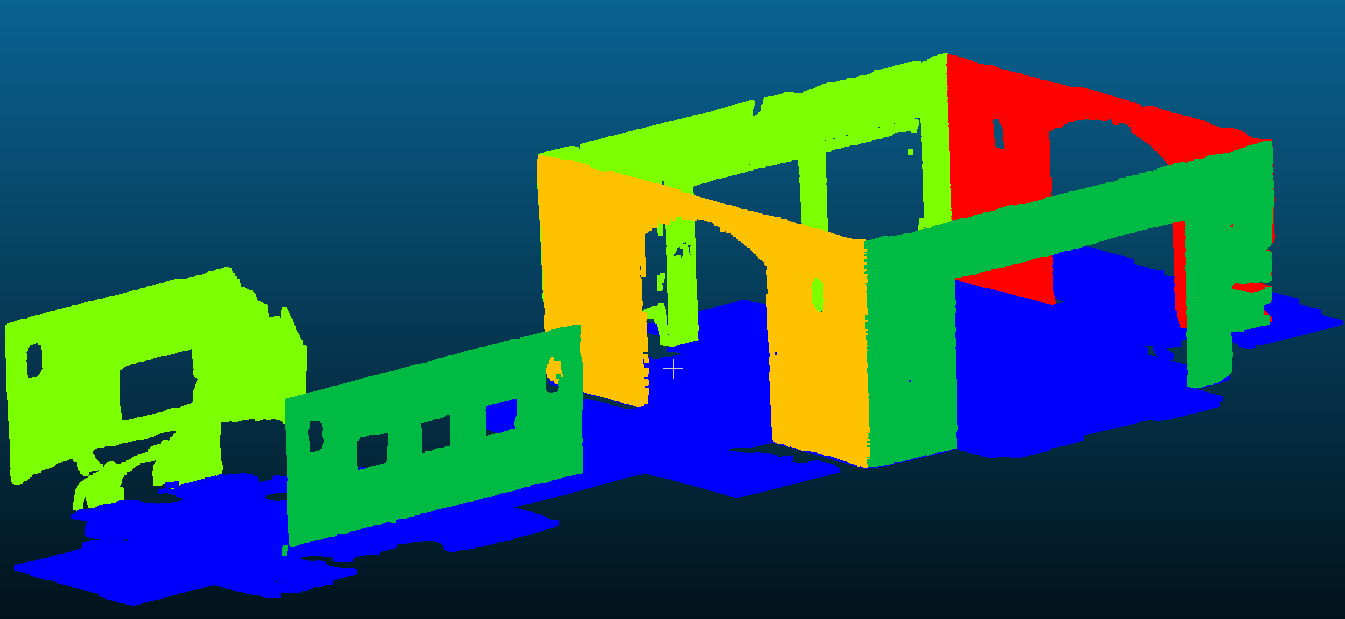
\includegraphics[width=0.3\linewidth]{figures/bonus_2.png}
    \caption{Segmentation with 5 planes, using a distance thrshold 0.2, an angle threshold of 10 degrees and 500 draws.
    Left: using the original method. Right: using the improved method.}
    \label{fig:bonus_2}
\end{figure}

Since one of the inlier criterions involves the distance to the plane, a strategy could be to perform a KDTree radius query at regular positions on the candidate plane. This would enable to consider only points which already verify
the distance condition, and may significantly speed up computation and save memory. However, our available implementation of the KDTree is CPU limited and too slow to speed-up anything. Better data structure may be preferable.


\end{document}

